\documentclass[a4paper,openright,11pt]{article}
\date{}
\usepackage[spanish]{babel}
\usepackage{graphicx}
\usepackage{amssymb}
\usepackage{fancyhdr}
\usepackage{multirow}
\usepackage[utf8]{inputenc}
\usepackage{fancyhdr}
\usepackage{float}
\usepackage{color}
\usepackage{listings}

\begin{document}
\renewcommand{\tablename}{Tabla}
\renewcommand{\listtablename}{\'Indice de tablas}
\renewcommand{\headrulewidth}{0.3pt}
\renewcommand{\footrulewidth}{0.3pt}
\newpage

\begin{titlepage}
	\begin{center}
		\vspace*{-1in}
		\begin{figure}[htb]
			\begin{center}
				
\includegraphics[width=10cm]{ug}
			\end{center}
		\end{figure}
		\vspace*{0.1in}
		\begin{Large}
			Ingenier\'ia en Sistemas, Inform\'atica y \\Ciencias de la Computaci\'on\\
		\end{Large}
		\vspace*{0.2in}
		\begin{Large}
			Seminario Profesional II\\
		\end{Large}
		\vspace*{0.9in}
		\begin{LARGE}
			\textbf{\LARGE MAYALENG} \\
			\begin{figure}[htb]
				\begin{center}
					
\includegraphics[width=4cm]{ml}
				\end{center}
			\end{figure}
		\end{LARGE}
		\vspace*{0.9in}
		\begin{large}
			Autores:\\
			Douglas Figueroa \\
			Alexander Baquiax
		\end{large}
		\vspace*{0.3in}
		\\
		\rule{90mm}{0.1mm}\\
		\begin{large}
			Supervisado por: \\
			Ing. Jack Trachtenberg \\
			Ing. Axel Benavides
		\end{large}
	\end{center}
\end{titlepage}
\newpage

\tableofcontents

\cleardoublepage
\listoffigures

\cleardoublepage
\listoftables

\newpage

\pagestyle{fancy}
\rfoot{
\includegraphics[width=.08\textwidth]{ml}}
\lfoot{MayaLeng}
\section{Introducci\'on}
Mayaleng más que una aplicación es un algoritmo con la capacidad de recibir un input, en nuestro caso, una palabra, una frase, un párrafo, una cantidad de texto muy grande, en español y retornar un output, (el texto de entrada), en una lengua maya. \\

Una herramienta de traducción y para conocimiento de la cultura de Guatemala.\\

La cultura en Guatemala es muy grande, uno de los propósitos de este proyecto es poder aportar a expandir el conocimiento en las lenguas mayas, una rama que forma gran parte de la cultura, por medio de un algoritmo de traducción, utilizando diferentes tecnologías, hacemos dicho aporte, creando un traductor de español e inglés a una lengua maya, el Kaqchikel.\\

Una aplicación móvil y web nos ayudará a expandir el conocimiento de esta lengua maya, la tecnología cada vez es más accesible, los teléfonos inteligentes y las computadores cada vez son más comunes en los hogares, lo que nos ayuda a deducir que el alcance puede ser mayor. Pero no solamente estamos enfocando esta herramienta al uso particular de personas, también se enfoca a que sea una herramienta de trabajo para quienes enseñan a otros el español, en este caso es un profesor quien utiliza la herramienta y es cierto que esta persona ya conoce la lengua maya pero con la herramienta puede generar su propia documentación para los alumnos que este tenga.\\

Utilizamos muchas herramientas para la construccións de este proyecto, MySQL, LiguaKit, PHP, Symfony, Ionic, API's; herramientas de las cuales iremos hablando en el desarrollo del proyecto.
\newpage

\section{Objetivos}
\subsection{Objetivo General}
Crear una herramienta de traducci\'on de la lengua maya Kaqchikel.
\subsection{Objetivos Espec\'ificos}
\begin{itemize}
    \item Crear una aplicaci\'on m\'ovil (Android y iOS) para traducción del Kaqchikel.
    \item Dar a conocer la cultura de nuestro pa\'is Guatemala.
    \item Brindar la capacidad a profesores y personas en general de traducir documentos para facilitar su trabajo en los lugares d\'onde imparten clases dentro de nuestro pa\'is y los cuales no dominan el espa\~nol.
\end{itemize}
\newpage

\section{El Problema}
\subsection{¿Cuál es el problema?}
El problema analizado para querer desarrollar esta herramienta fue desde un punto de vista cultural, ya que en Guatemala existen muchas lenguas mayas, de las cuales pocas personas en el pa\'is dominan como m\'inimo una. Estas forman parte de nuestro patrimonio cultural. Alrededor del mundo Guatemala es conocida por los puntos tur\'isticos con los que contamos, regularmente estos se encuentran en los departamentos donde al menos existe una lengua Maya.  Como guatemaltecos deber\'iamos de poder comunicarnos con la gente de nuestro pa\'is, ya que en algunos departamentos no se habla mucho en espa\~nol sino que hablan en una lengua maya, sin embargo ese no es el caso. No hemos encontrado tantas herramientas claras que nos faciliten dicha tarea, queremos ser de los primeros en brindar dicha herramienta.\\

En este momento sugerimos Kaqchikel, la forma en que solucionamos el problema de la comunicación es teniendo una aplicación m\'ovil la cu\'al har\'a una traducción en nuestro idioma natal a Kaqchikel, sencillamente quien utilice la aplicación deberá ingresar el texto y en una casilla aparte aparecer\'a la traducci\'on del texto, algo similar a google translate.\\

Le ahorraremos al usuario tener que escribir algunas de las frases o palabras m\'as utilizadas, ya que tendremos una secci\'on donde diremos como se dicen esas frases, cosas b\'asicas como saludar, despedirse, hasta algo m\'as formal, un ejemplo ser\'ia preguntar d\'onde se encuentra el bano, preguntar el nombre de una persona y frases similares.\\
\newpage

\section{Estudio de Factibilidad}
\subsection{Factibilidad Funcional}
\subsubsection{Resultados de Encuesta}
\begin{figure}[H]
	\centering
	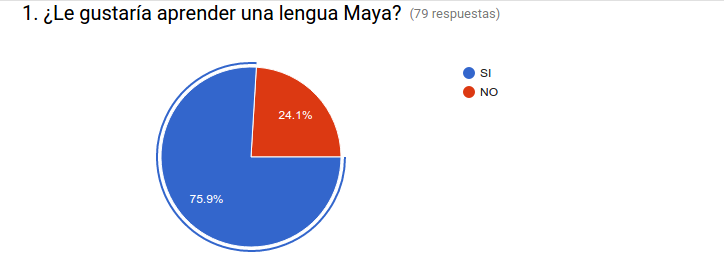
\includegraphics[width=1.0\textwidth]{e1}
	\caption{Aprender una lengua maya}
	\label{fig:e1}
	Del total de personas que contestaron la encuesta podemos observar que poco más del 75\% de las personas está interesada en aprender una lengua mayal.
\end{figure}
\begin{figure}[H]
	\centering
	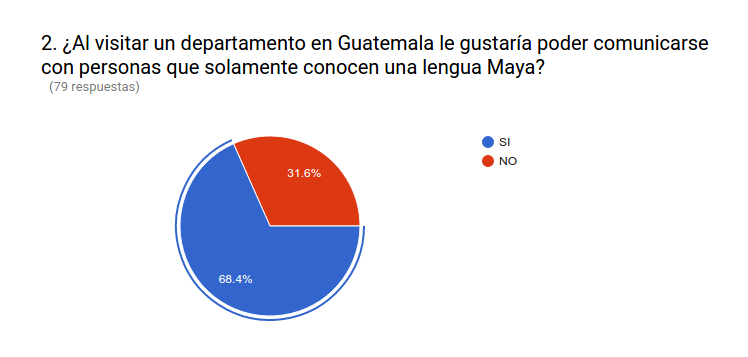
\includegraphics[width=1.0\textwidth]{e2}
	\caption{Comunicación en lengua maya}
	\label{fig:e2}
	En la gráfica podemos observar que casi la tercera parte de las personas les gustaría entablar una conversación en lengua maya, estas personas pueden estar enlazadas a la pregunta 1, que contestaron con un sí.
\end{figure}
\begin{figure}
	\centering
	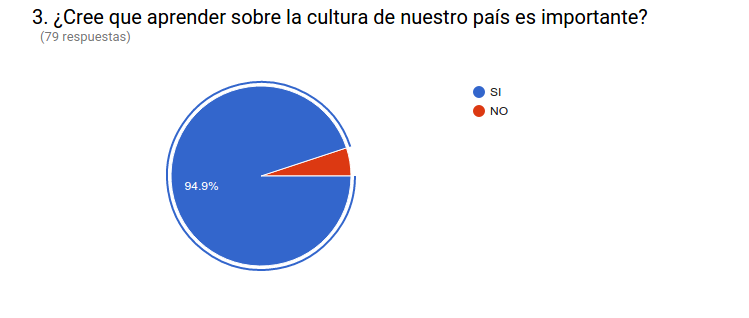
\includegraphics[width=1.0\textwidth]{e3}
	\caption{Cultura importante}
	\label{fig:e3}
	En esta pregunta vemos que casi todos contestaron que sí, hay un pequeño porcentaje que piensa que la cultura de nuestro país no es algo importante.
\end{figure}
\begin{figure}
	\centering
	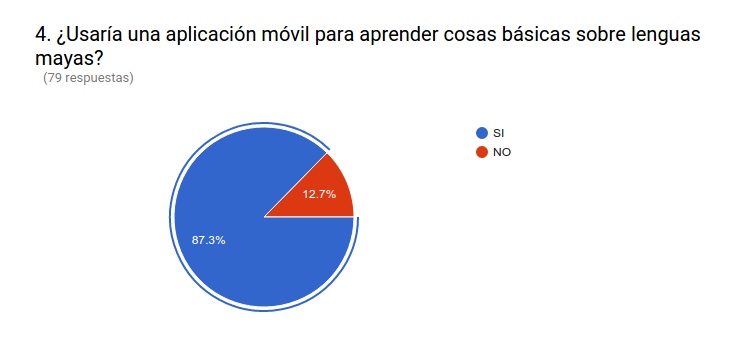
\includegraphics[width=1.0\textwidth]{e4}
	\caption{Una aplicación móvil}
	\label{fig:e4}
	Todas las personas que entrevistamos cuentan con un smartphone, de todas esas personas la mayoría está dispuesta a instalar y utilizar nuestra aplicación en su teléfono.
\end{figure}
\begin{figure}
	\centering
	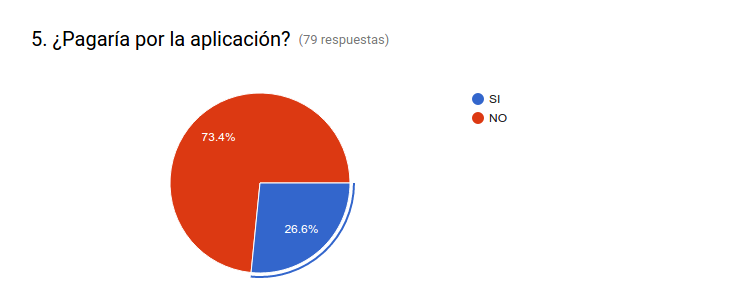
\includegraphics[width=1.0\textwidth]{e5}
	\caption{Pago por la apliación}
	\label{fig:e5}
	En esta pregunta creímos que el 100\% de las personas contestaría con un no, sin embargo un pequeño porcentaje de personas estaría dispuesta a pagar por la aplicación.
\end{figure}
\begin{figure}
	\centering
	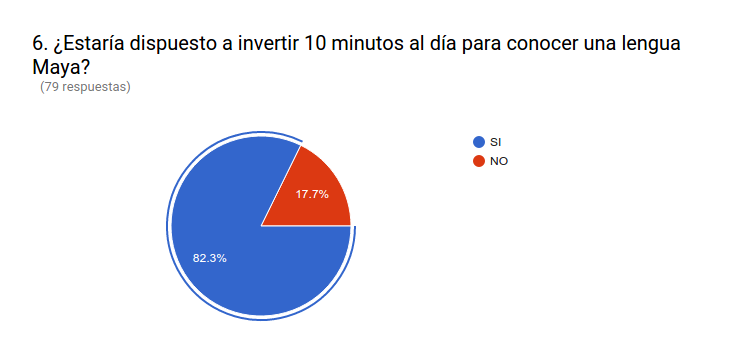
\includegraphics[width=1.0\textwidth]{e6}
	\caption{Inversión de tiempo}
	\label{fig:e6}
	Diez minutos es un pequeño tiempo para revisar una aplicación móvil, tiempo que la mayoría de los entrevistados estarían dispuestos a utilizar para revisar el traductor maya.
\end{figure}

\subsubsection{Tablas Comparativas}
\begin{table}[H]
	\resizebox*{14cm}{!}{
	\begin{tabular}{|r|c|c|c|c|}
	\hline
	Funcionalidad & Google Translate & Glosbe.com & Profesor & MayaLeng\\
	\hline
	Traducci\'on de palabras & \checkmark & \checkmark & \checkmark & \checkmark\\
	\hline
	Traducci\'on	 bidireccional & \checkmark & x & \checkmark & x\\
	\hline
	Traducci\'on de frases  & \checkmark & x & \checkmark & \checkmark\\
	\hline
	Traducci\'on precisa & \checkmark & x & \checkmark & \checkmark\\
	\hline
	Herramienta de traducci\'on de documentos & \checkmark & x & \checkmark & \checkmark\\
	\hline
	\end{tabular}}
\caption{Comparativa de Funcionalidades}
	A nivel de funcionalidad nuestro competidor más grande es un profesor, quién posee las habilidades necesarias para desempeñar el trabajo de traductor, sin embargo hablamos de una persona contra una herramienta de tecnología que es más factible.
\end{table}

\begin{table}[H]
	\resizebox*{14cm}{!}{
	\begin{tabular}{|r|c|c|c|c|}
	\hline
	Caracter\'istica & Google Translate & Glosbe.com & Profesor & MayaLeng\\
	\hline
	Descripci\'on de palabras & x & \checkmark & \checkmark & x\\
	\hline
	Intuitivo & \checkmark & x & \checkmark & \checkmark\\
	\hline
	Es gratis  & \checkmark & \checkmark & x & \checkmark\\
	\hline
	Siempre disponible & \checkmark & \checkmark & x & \checkmark\\
	\hline
	F\'acil de obtener/contactar & \checkmark & \checkmark & x & \checkmark\\
	\hline
	\end{tabular}}
\caption{Comparativa de Caracter\'isticas}
Cuando evaluamos características la tecnología toma el control en aportar más cosas factibles que un profesor (nuestra mayor competencia), y podemos observar que MayaLeng cumple con casi todas las características de la evaluación realizada.
\end{table}

\subsubsection{Conclusión}
Nuestra herramienta cumple con ser una herramienta factible, en base a las encuestas, conocemos la opinión de las personas y vemos que comportamiento tendrían si tuvieses la herramienta en sus manos, con las tablas comparativas pudimos ver a que nivel nos encontramos comparándonos con otras soluciones similares.

\subsection{Factibilidad T\'ecnica}
Pretendemos aprovechar el apogeo de los m\'oviles y tratar de crear una buena oportunidad para introducir nuestro proyecto.\\
Actualmente existen dos grandes sistemas operativos que domina la industria de los m\'oviles:. iOS y Android. Estamos conscientes de que desarrollar de forma nativa para ambas plataformas nos representar\'ia un poco m\'as de tiempo, que implicar\'ia restarle tiempo a la parte que en verdad es importante. Por lo cual usaremos IONIC, framework que nos permite desarrollar de manera sencilla aplicaciones m\'oviles usando las tendencias de Responsive Web Design. \\

Lo interesante de este proyecto no radica en la aplicaci\'on m\'ovil, de hecho la aplicaci\'on s\'olo ser\'a una forma de consumir nuestro verdadero sistema.\\

La idea de este proyecto radica en hacer un compilador que pueda usar una gram\'atica y una fuente de palabras de esa gram\'atica, y traducir de ellas las palabras al español. En pocas palabras nuestro proyecto radica en hacer un compilador de idiomas mayas.\\

Durante el transcurso de nuestra carrera ya hicimos un compilador, con todas las fases b\'asicas que uno de ellos debe tener. Ahora nos pusimos el reto de hacer un compilador gen\'erico. Para esta primera versi\'on usaremos dos idiomas Mayas.\\

Creemos tener los conocimientos necesarios para la construcci\'on de esto. Uno de los inconvenientes m\'as grandes era que ninguno de los dos sabemos hablar un idioma Maya, pero nos apoyamos en la documentaci\'on que distintas personas a lo largo de la historia han construido.\\ 

La idea es construir un API al que se le pueda dar como input un texto, p\'arrafo, documento y que la salida sea otro documento pero con texto traducido. Ahora tenemos una base de datos con 15 mil palabras aproximadamente del Kaqchikel. La DB esta montada en un DBMS MySQL. El API fue construido en Symfony2.\\

El core de traducci\'on ser\'a hecho en Java,  usando herramientas de parseo y an\'alisis sint\'actico como Flex.

\subsubsection{Conclusión}
La tecnología utilizada cubre con las necesidades para el proyecto, nos ayuda a que las tareas sean optimizadas, utilizando menos recursos y optimización de tiempo, lo cuál es un punto muy importante a considerar.

\subsection{Factibilidad Econ\'omica}
Bas\'andonos en nuestra calendarizaci\'on de tareas para el desarrollo del proyecto, hemos estimado los siguientes costos para el desarrollo de la aplicaci\'on, los gastos son a nivel de costo de servidor, por compra del dominio, licencias para subir aplicaci\'on y gastos en papel, en impresi\'on del manual de usuario.\\

\begin{table}[h]
	\resizebox*{15cm}{!}{
	\begin{tabular}{|l|c|r|}
	\hline
	Tarea & D\'ias Trabajados & Costo (Q.)\\
	\hline
	Configurar servicios iniciales.\\
	Montar la base de datos del proyecto anterior.
	& 7 
	& 70\\
	\hline
	Generar la documentación adecuada del algoritmo de traducción.\\
	Extraer las reglas de la gramática de libros y textos.
	& 7 
	& 130\\
	\hline
	Lanzar primera versión del API.\\
	Traducción de oraciones sencillas.\\
	App consumiendo API.
	& 7
	& 192\\
	\hline
	Documentación final y manual de usuario.\\
	Lanzamiento final.
	& 7
	& 50\\
	\hline
	Total 
	&
	& 442\\
	\hline
	\end{tabular}}
\caption{Factibilidad Econ\'omica}
\end{table}

\subsubsection{Conclusión}
El costo monetario del desarrollo de nuestra herramienta no es tan alto debido a qué contamos con las herramientas para prueba (teléfono con Android y iPad) y pocas cosas son en las que hemos invertido.
\newpage

\section{Marco Teórico}
\subsection{Lenguas Mayas}
En Guatemala contamos actualmente con más de 20 lenguas mayas,  los Acuerdos de Paz firmados en diciembre de 1996 hacen un compromiso de estado, el reconocimiento de los diferentes idiomas del país, lo cual hace que el país sea reconocido como uno multilingüe, y se hace constar en la Constitución que los idiomas mayas deberán respetarse y difundirse. Se han hecho esfuerzos, sin embargo los pocos habitantes que quedan hacen difícil la tarea. Muchos jóvenes de las nuevas generaciones no llegan a aprender el idioma indígena de sus padres. Actualmente los idiomas de mayor habla son el Kekchí, el Quiché, el Kaqchikel, el Mam y el Tzutujil, los cuales tienen algunos vocablos y reglas gramaticales en común. \\
 
Las lenguas mayenses derivan del protomaya, una protolengua (reconstrucción probable de la lengua origen de un grupo de lenguas), que pudo haberse hablado hace unos 5000 años a juzgar por el grado de diversificación interna en una región cercana a donde actualmente se hablan lenguas mayenses.

\begin{figure}[H]
	\centering
	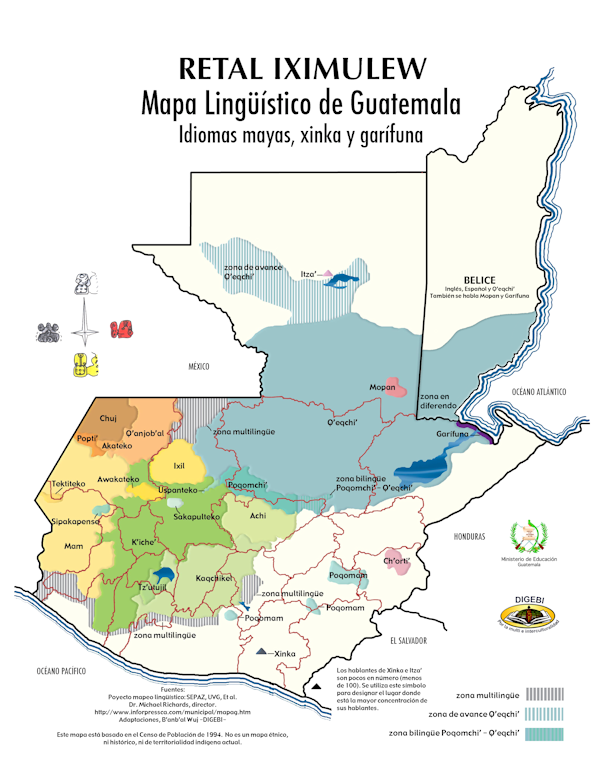
\includegraphics[width=0.6\textwidth]{mapa}
	\caption{Mapa de lenguas mayas}
	Las lenguas mayas están distribuidas por todo el país.
	\label{fig:map}
\end{figure}

\begin{figure}[H]
	\centering
	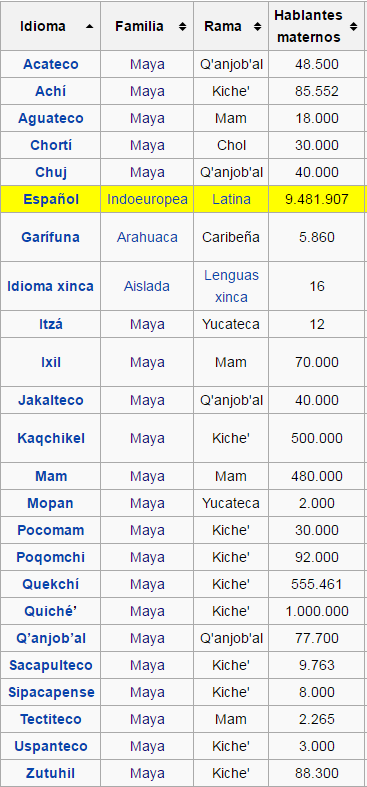
\includegraphics[width=0.6\textwidth]{tablalenguas}
	\caption{Tabla de lenguas mayas}
	Cantidad de hablantes de cada lengua.
	\label{fig:tabla}
\end{figure}

\begin{figure}[H]
	\centering
	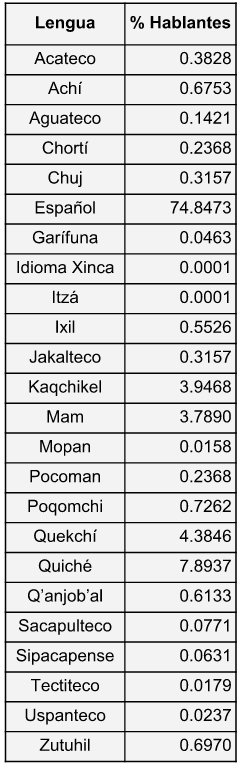
\includegraphics[width=0.3\textwidth]{porhablantes}
	\caption{Porcentaje de hablantes de lenguas mayas}
	\label{fig:porc}
\end{figure}

Como parte de las herramientas involucradas para el desarrollo de este proyecto tenemos:\\
\begin{table}[H]
	\begin{center}
	\resizebox*{5cm}{!}{
		\begin{tabular}{|l|l|}
			\hline
			1. & MySQL\\
			\hline
			2. & PHP\\
			\hline
			3. & RAE\\
			\hline
			4. & RAE\\
			\hline
			5. & LinguaKit\\
			\hline
			6. & Symfony\\
			\hline
			7. & Ionic\\
			\hline
			8. & Formularios de Google\\
			\hline
			9. & LaTex\\
			\hline
			10. & Wordpress\\
			\hline
		\end{tabular}}
	\end{center}
	\caption{Tecnologías Involucradas}
\end{table}


Habíamos mencionado en la sección 3, \textbf{\textit{El Problema}}, que nuestra problemática era desde un punto cultural, un problema de comunicación interna por falta de conocimiento, porque no conocemos las lenguas mayas, no las podemos hablar, y tampoco encontramos información fácil sobre ellas, no es cómo hacer una traducción en Google translate y saber como se escribe alguna palabra que necesitamos usar, eso nos lleva al siguiente análisis. \\

\newpage

\section{MayaLeng}
\textbf{\textit{¿En qué consiste?}}\\
La solución planteada a esta problemática es la construcción de un algoritmo que nos ayude a establecer esta comunicación que no se posee, trabajamos en un traductor con el cual podamos transformar frases en español a frases en una lengua maya, como lengua inicial hemos escogido el Kaqchikel. Una vez construido el algoritmo de traducción necesitamos un dispositivo por el cual podamos darle uso a dicha herramienta, el dispositivo que elegimos para nuestra implementación es un teléfono inteligente, lo aplicamos para teléfonos que tengan instalado los sistemas operativos \textbf{Android} y \textbf{iOS}; Android es un sistema operativo móvil creado por Google Inc, y iOS es un sistema operativo móvil creado por Apple Inc.\\

El mercado de teléfonos inteligentes cada vez crece más, con la llegada del 4G el mercado móvil dió un nuevo paso y más personas tienen más fácil acceso al internet por medio de un dispositivo móvil, por lo que tener aplicaciones que requieran internet cada vez es menos costoso para el usuario, en el 2014 se estimó que había una cantidad de 21.7 millones de líneas telefónicas móvil en el país.\\

\textbf{\textit{¿Qué hicimos?}}\\
Creamos una aplicación móvil con el nombre de \textbf{\textit{MayaLeng}} utilizando \textbf{ionic}, este es un framework que nos permite hacer un solo desarrollo y compilar nuestro programa una sola vez y generaramos una aplicación para iOS y Android; MayaLeng consume el algoritmo de traducción.\\\\

\textbf{\textit{¿Cómo funciona?}}\\
Lo que se requiere para su funcionamiento es escribir una palabra, una frase, una oración o un párrafo en una caja de texto, una vez MayaLeng haya iniciado, este texto llega al algoritmo, contamos con un diccionario de español-kaqchikel, el diccionario lo llenamos con su respectivo tipo de palabra, el cual obtuvimos utilizando la \textbf{RAE}, una institución cultural dedicada a la regularización lingüística.\\ 
Utilizamos su API con un scritp desarrollado en \textbf{PHP} que es un lenguaje de programación que se ejecuta del lado del servidor, es considerado uno de los lenguajes más flexibles, potentes y de alto rendimiento,  con este script obtenemos el tipo de palabra (sustantivo, pronombre, verbo, etc) de cada una de las contenidas en el diccionario.\\ 
El diccionario está almacenado en una base de datos \textbf{MySQL} que es sistema gestor de base de datos (DBMS) de licencia gratuita; mandamos nuestra oración a otra herramienta llamada \textbf{LinguaKit} que nos devuelve cada palabra de nuestra oración con su respectivo tipo de palabra. Las palabras podrían ser artículo, pronombre, verbos; una vez tenemos esos resultados los enlazamos con el tipo de palabra con el que ya contamos en la base de datos y ya teniendo la información, con \textbf{Symfony}, un framework diseñado para optimizar el desarrollo de las aplicaciones web basado en el patrón MVC (Modelo Vista Controlador), construímos la oración.\\\\

\textit{\textbf{¿Cómo construímos la oración?}}\\
Para explicar la construcción mostramos la siguiente imagen:\\
\begin{figure}[H]
	\centering
	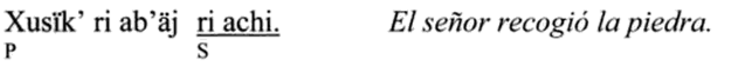
\includegraphics[width=0.6\textwidth]{oracion}
	\caption{Oración español-kaqchikel}
	\label{fig:kaq}
\end{figure}
La estructura de una oración simple en español es:
\begin{center}
	\textit{Sujeto - Predicado}\\
\end{center}

La estructura de una oración simple en Kaqchikel es:
\begin{center}
	\textit{Predicado - Sujetio}\\
\end{center}

Basándonos en la respuesta de \textit{Linguakit}, que nos devuelve que palabras forman parte del sujeto, y cuales del predicado, podemos colocar cada palabra en su orden correspondiente en base a la estructura de Kaqchikel que se obtuvo, este procedimiento lo realizamos para oraciones simples.

\subsection{Diagrama Entidad-Relación}
\begin{figure}[h]
	\centering
	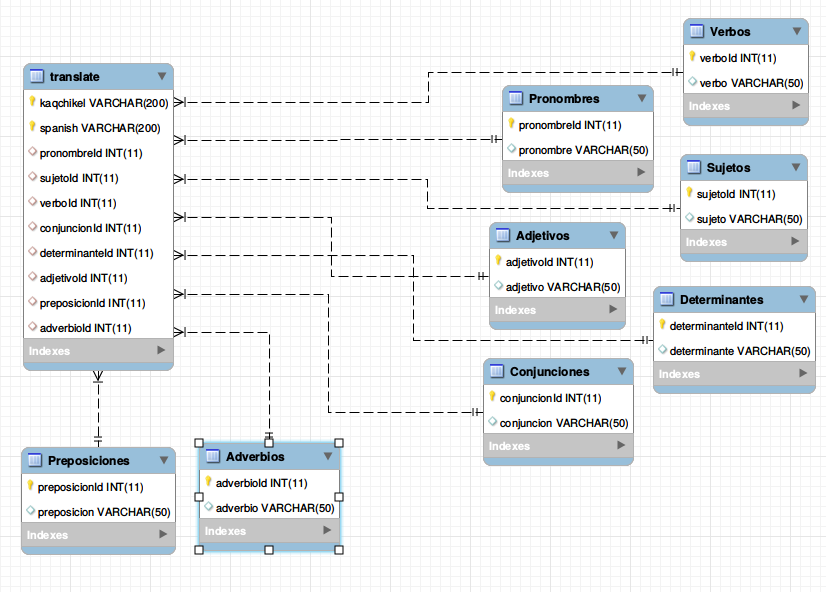
\includegraphics[width=0.9\textwidth]{er}
	\caption{Diagrama Entidad Relación}
	\label{fig:er}
\end{figure}
La base de datos está compuesta por una tabla principal que contiene el vocabulario, con la palabra en español y su traducción a Kaqchikel, una tabla con la estructura gramatical (sujeto, verbo, adjetivo, etc), y una tercer tabla que nos servirá para enlazar nuestro vocabulario con el tipo de palabra a la que aplique (por ejemplo: él=pronombre).\\
En nuestro diagrama está contemplado el caso que una palabra pudiese cumplir con más de una regla gramatical, y nos es posible almacenar esa información con nuestra tercer tabla donde tenemos las llaves primarias de cada tabla por lo cual no nos toparíamos con ningún registro duplicado.

\subsection{Diagrama de Arquitectura}
\begin{figure}[h]
	\centering
	\includegraphics[width=0.9\textwidth]{arquitectura}
	\caption{Diagrama de Arquitectura}
	\label{fig:arq}
\end{figure}
Gráfico de arquitectura de MayaLeng donde explicamos cómo está construido nuestro proyecto, dividido en dos partes principales que constan de la información, que cuenta con nuestro vocabulario, la base de datos, un servicio de migración utilizando la RAE, y el API, el cual divide las oraciones y construye las nuevas en el nuevo lenguaje.

\subsection{Diagrama de Arquitectura con Tecnologías}
\begin{figure}[H]
	\centering
	\includegraphics[width=0.9\textwidth]{arquitecturalogos}
	\caption{Diagrama de Arquitectura Logos} 
	Tecnologías utilizadas
	\label{fig:arqL}
\end{figure}

\subsection{Diagrama de Secuencia - Palabra}
\begin{figure}[h]
	\centering
	\includegraphics[width=0.9\textwidth]{secuencia}
	\caption{Diagrama de Secuencia}
	\label{fig:sec}
\end{figure}
Aquí se presenta el flujo que tiene una palabra al ser ingresada por el usuario hasta regresar de nuevo pero ya traducida.

\subsection{Diagrama de Secuencia - Oraciones}
\begin{figure}[H]
	\centering
	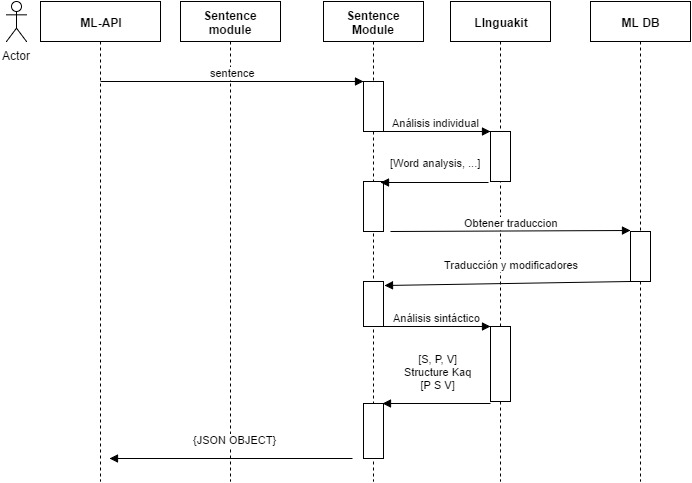
\includegraphics[width=0.9\textwidth]{secuenciaoracion}
	\caption{Diagrama de Secuencia de Oraciones}
	\label{fig:seco}
\end{figure}

\subsection{Diagrama de Casos de Uso}
\begin{figure}[h]
	\centering
	\includegraphics[width=0.6\textwidth]{casouso}
	\caption{Diagrama de Caso de Uso}
	\label{fig:caso}
\end{figure}
\newpage

\subsection{Algoritmos implementados}
\subsubsection{Traducción de español a kaqchikel}
Lo que realiza este algoritmo, el cual es una implementación propia, se describe a continuación:

\begin{lstlisting}
Recibe texto
Si TextoMuyLargo Entonces
	Descomponer en oraciones mas cortas
	
Obtener palabras de texto
Mientras Palabras > 0
	Obtener traduccion de cada palabra en kaqchikel
	
Analizar tipo de palabra
Analizar estructura de oracion en kaqchikel
Armar nuevo texto
Devolver nuevo texto
\end{lstlisting}
\newpage

\section{Conclusiones}
\begin{itemize}
	\item Aprendimos un poco más de la cultura de Guatemala, sobre las lenguas mayas.
	\item Pusimos en práctica varios temas de los aprendidos en la Universidad.
	\item Aprendimos nuevas tecnologías.
\end{itemize}
\newpage

\section{Recomendaciones}
\begin{itemize}
	\item Aprender más sobre la cultura de Guatemala.
\end{itemize}
\newpage

\section{Referencias}
\begin{itemize}
	\item Filiberto Patal Majzul. (2007). Ruzoltzij Ri Kaqchikel. Guatemala|: Cholsamaj.
	\item (2006). Lenguas mayenses. 2006, de Wikipedia Sitio web: http://bit.ly/2dTGuVy
	\item (2002). Lenguas de Guatemala. 2002, de Wikipedia Sitio web: http://bit.ly/2fuwPpd
\end{itemize}
\newpage

\section{Anexo}
\subsection{Calendarización}
\begin{figure}[h]
  \centering
    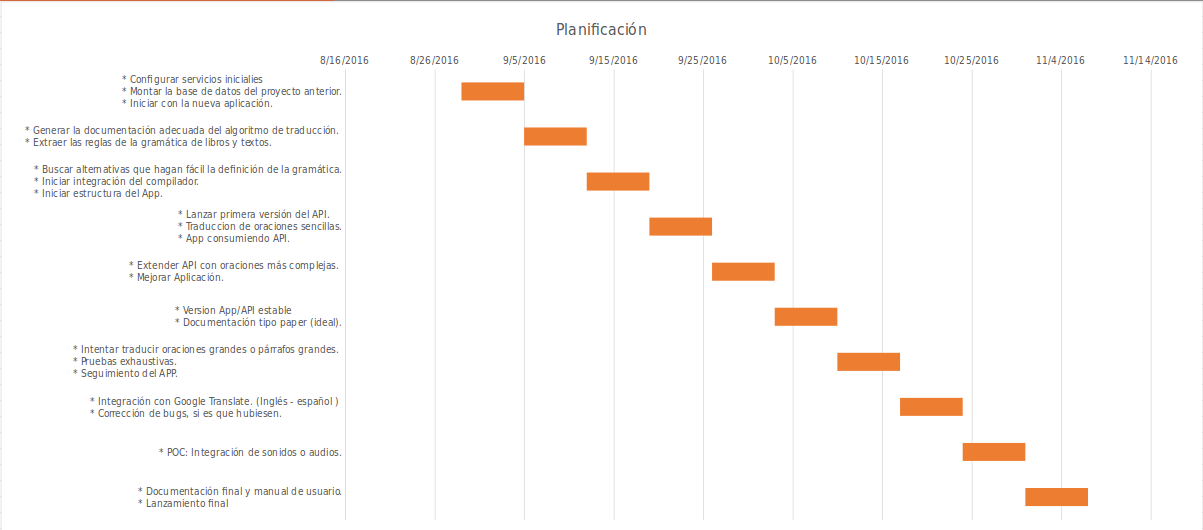
\includegraphics[width=1.0\textwidth]{Gantt}
  \caption{Diagrama de Gantt}
  \label{fig:gantt}
\end{figure}

\subsection{Encuesta}
\begin{enumerate}
	\item ¿Le gustaría aprender una lengua maya?\\
	SI \rule{10mm}{0.1mm}  \hspace{5cm} NO \rule{10mm}{0.1mm}
	\item ¿Al visitar un departamento en Guatemala le gustaría poder comunicarse con personas que solamente conocen una lengua maya?	\\
	SI \rule{10mm}{0.1mm}  \hspace{5cm} NO \rule{10mm}{0.1mm}
	\item ¿Cree que aprender sobre la cultura de nuestro país es importante?\\
	SI \rule{10mm}{0.1mm}  \hspace{5cm} NO \rule{10mm}{0.1mm}
	\item ¿Usaría una aplicación móvil para aprender cosas básicas sobre lenguas mayas?\\
	SI \rule{10mm}{0.1mm}  \hspace{5cm} NO \rule{10mm}{0.1mm}
	\item ¿Pagaría por la aplicación?\\
	SI \rule{10mm}{0.1mm}  \hspace{5cm} NO \rule{10mm}{0.1mm}
	\item ¿Estaría dispuesto a invertir 10 minutos al día para conocer una lengua maya?\\
	SI \rule{10mm}{0.1mm}  \hspace{5cm} NO \rule{10mm}{0.1mm}
\end{enumerate}
\newpage

\section{Glosario}
\noindent \textbf{Kaqchikel: } lengua maya, parte de la familia lingüística mayense. \\\\
\textbf{iOS: } sistema operativo móvil de Apple \\\\
\textbf{Android: } sistema operativo móvil de Google \\\\
\textbf{Framework: } conjunto estandarizado de conceptos, prácticas y criterios para enfrentar y resolver nuevos problemas de índole similar. \\\\
\textbf{Responsive Web Design:  adaptar la apariencia de las páginas web al dispositivo que se esté utilizando para visualizarlas. }  \\\\
\textbf{API:  } utilizada por otro software como una capa de abstracción \\\\
\textbf{DB: } base de datos \\\\
\textbf{DBMS: } programa que permite almacenar y posteriormente acceder a los datos de forma rápida y estructurada.\\\\
\textbf{MySQL: }  sistema de gestión de bases de datos relacional \\\\
\textbf{Symfony2: } framework diseñado para optimizar el desarrollo de aplicaciones web\\ \\
\newpage

\pagestyle{fancy}
\end{document}